\chapter{Deep Learning}

\section*{Introduction}
    Dans ce chapitre, je vais vous présenter ce qu'est le deep learning et ce que sont les réseaux de neurones, et surtout la différence entre les différentes méthodes de classification d'images
\section{Géneralité}
    \subsection{Definition}
        \begin{enumerate}
            \item \textbf{Machine Learning (ML):} 
            
            Selon Wikipedia L'apprentissage automatique est un champ d'étude de l'intelligence artificielle qui se fonde sur des approches mathématiques et statistiques pour donner aux ordinateurs la capacité d'« apprendre » à partir de données, c'est-à-dire d'améliorer leurs performances à résoudre des tâches sans être explicitement programmés pour chacune. Plus largement, il concerne la conception, l'analyse, l'optimisation, le développement et l'implémentation de telles méthodes.


            \item \textbf{Deep Learning (DL):} 
            
            Selon Wikipedia L'apprentissage profond est un ensemble de méthodes d'apprentissage automatique tentant de modéliser avec un haut niveau d’abstraction des données grâce à des architectures articulées de différentes transformations non linéaires. Ces techniques ont permis des progrès importants et rapides dans les domaines de l'analyse du signal sonore ou visuel et notamment de la reconnaissance faciale, de la reconnaissance vocale, de la vision par ordinateur, du traitement automatisé du langage. Dans les années 2000, ces progrès ont suscité des investissements privés, universitaires et publics importants, notamment de la part des GAFAM (Google, Apple, Facebook, Amazon, Microsoft).
        \end{enumerate}
    \subsection{Historique}
        Depuis l'antiquité, le sujet des machines pensantes préoccupe les esprits. Ce concept est la base de pensées pour ce qui deviendra ensuite l'intelligence artificielle, ainsi qu'une de ses sous-branches : l'apprentissage automatique.
        La concrétisation de cette idée est principalement due à Alan Turing (mathématicien et cryptologue britannique) et à son concept de la « machine universelle » en 1936, qui est à la base des ordinateurs d'aujourd'hui. Il continuera à poser les bases de l'apprentissage automatique, avec son article sur « L'ordinateur et l'intelligence » en 1950, dans lequel il développe, entre autres, le test de Turing.
        En 1943, le neurophysiologiste Warren McCulloch et le mathématicien Walter Pitts publient un article décrivant le fonctionnement de neurones en les représentant à l'aide de circuits électriques. Cette représentation sera la base théorique des réseaux neuronaux.
        Arthur Samuel, informaticien américain pionnier dans le secteur de l'intelligence artificielle, est le premier à faire usage de l'expression machine learning (en français, « apprentissage automatique ») en 1959 à la suite de la création de son programme pour IBM en 1952. Le programme jouait au Jeu de Dames et s'améliorait en jouant. À terme, il parvint à battre le 4e meilleur joueur des États-Unis.
        Une avancée majeure dans le secteur de l'intelligence machine est le succès de l'ordinateur développé par IBM, Deep Blue, qui est le premier à vaincre le champion mondial d'échecs Garry Kasparov en 1997. Le projet Deep Blue en inspirera nombre d'autres dans le cadre de l'intelligence artificielle, particulièrement un autre grand défi : IBM Watson, l'ordinateur dont le but est de gagner au jeu Jeopardy!. Ce but est atteint en 2011, quand Watson gagne à Jeopardy! en répondant aux questions par traitement de langage naturel.
        Durant les années suivantes, les applications de l'apprentissage automatique médiatisées se succèdent bien plus rapidement qu'auparavant.
        En 2012, un réseau neuronal développé par Google parvient à reconnaître des visages humains ainsi que des chats dans des vidéos YouTube.
        En 2014, 64 ans après la prédiction d'Alan Turing, le dialogueur Eugene Goostman est le premier à réussir le test de Turing en parvenant à convaincre 33 \% des juges humains au bout de cinq minutes de conversation qu'il est non pas un ordinateur, mais un garçon ukrainien de 13 ans.
        En 2015, une nouvelle étape importante est atteinte lorsque l'ordinateur « AlphaGo » de Google gagne contre un des meilleurs joueurs au jeu de Go, jeu de plateau considéré comme le plus dur du monde.
        En 2016, un système d'intelligence artificielle à base d'apprentissage automatique nommé LipNet parvient à lire sur les lèvres avec un grand taux de succès.

\section{Réseau des neurones}
        un réseau de neurones est une structure qui aide l'ordinateur à imiter le processus d'apprentissage du cerveau humain, en collectant un certain nombre de nœuds liés par des poids,la manifestation la plus élémentaire d'un réseau de neurones est ce qu'on appelle le perceptron, il s'agit d'un réseau de neurones à une seule couche composé de deux entrées et d'une sortie comme suit:

        \subsection{Perceptron}
            Comme mentionné ci-dessus, le perceptron est  un lien neuronal à une seule couche avec quatre paramètres principaux. Le modèle perceptron multiplie d'abord toutes les valeurs d'entrée et leurs poids, puis ajoute ces valeurs pour créer une somme pondérée. En outre, cette somme pondérée est appliquée à la fonction d'activation "f" pour obtenir la sortie souhaitée. Cette fonction d'activation est également appelée fonction échelon et est désignée par la lettre "f".
            \begin{figure}[h]
                \centering
                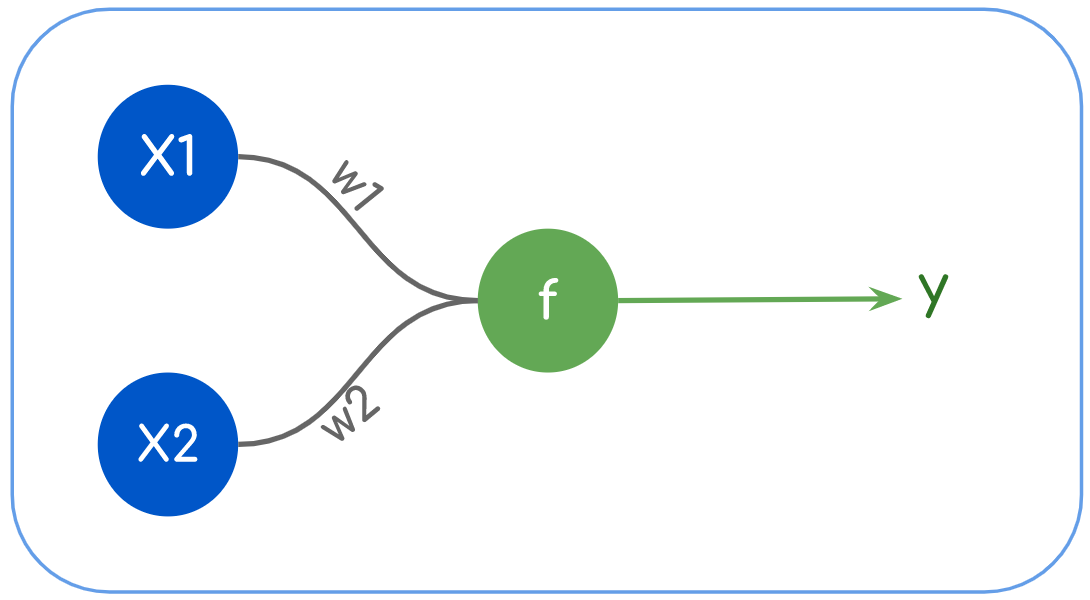
\includegraphics[scale=0.3]{perceptron}
                \caption{Perceptron}
                \label{fig:perceptron}
            \end{figure}

            \begin{itemize}[label=$\bullet$]
                \item Xi: entrées.
                \item Wi: poids.
                \item f: fonction d'activation.
                \item y: sortie 
            \end{itemize}

            cette fonction d'activation est nécessaire pour s'assurer que la sortie est  mappée entre (0,1) ou (-1,1). Notez que le poids de l'entrée indique la force d'un nœud. De même, une valeur d'entrée donne la possibilité de décaler la courbe de la fonction d'activation vers le haut ou vers le bas.
            
            Étape 1: Calculez la somme pondérée en multipliant toutes les valeurs d'entrée par leurs valeurs de poids respectives et en les additionnant. La formule est:

            \begin{equation}\label{eq:per_sum}
                \Sigma = \Sigma wi*xi = w1*x1 + w2*x2 + w3*x3 + \dots
            \end{equation}
            \myequations{Somme pondérée des entrées par leur poids}


            Nous ajoutons un terme appelé biais « b » à cette somme pondérée pour améliorer les performances du modèle. 
            Étape 2: La fonction d'activation est appliquée à l'aide des sommes pondérées ci-dessus pour donner la sortie sous forme binaire ou des valeurs continues comme suit:


            \begin{equation}\label{eq:per_sum}
                Y = f(\Sigma + b)
            \end{equation}
            \myequations{Calcule de sortie}

            Étape 3: finalement pour améliorer la précision du perceptron il faut ajuster les poids suivants la relation:

            \begin{equation}\label{eq:per_weights}
                W_n = W_a + \alpha (y_r - Y) X
            \end{equation}
            \myequations{Equation de calcule des nouveaux poids}
            

            Avec \boldmath{\(W_n\)} le nouveau vecteur des poids, \textbf{\(W_a\)} le dernier vecteur de poids, \textbf{\(\alpha\)} est le pas d'apprentissage, \textbf{\(y_r\)} la sortie attendée (réele), \textbf{Y} est la sortie prévue par le perceptron et finalement \textbf{X} est le vecteur contenant les valeur courants des entrée.

        En bref, un réseau neuronal profond est une structure compliquée composée de plusieurs perceptrons interconnectés. Dans un réseau neuronal, nous avons trois unités principales, la couche d'entrée, la couche de sortie et la couche cachée contenant plusieurs couches interconnectées.
        
        \begin{figure}[H] 
            \centering
            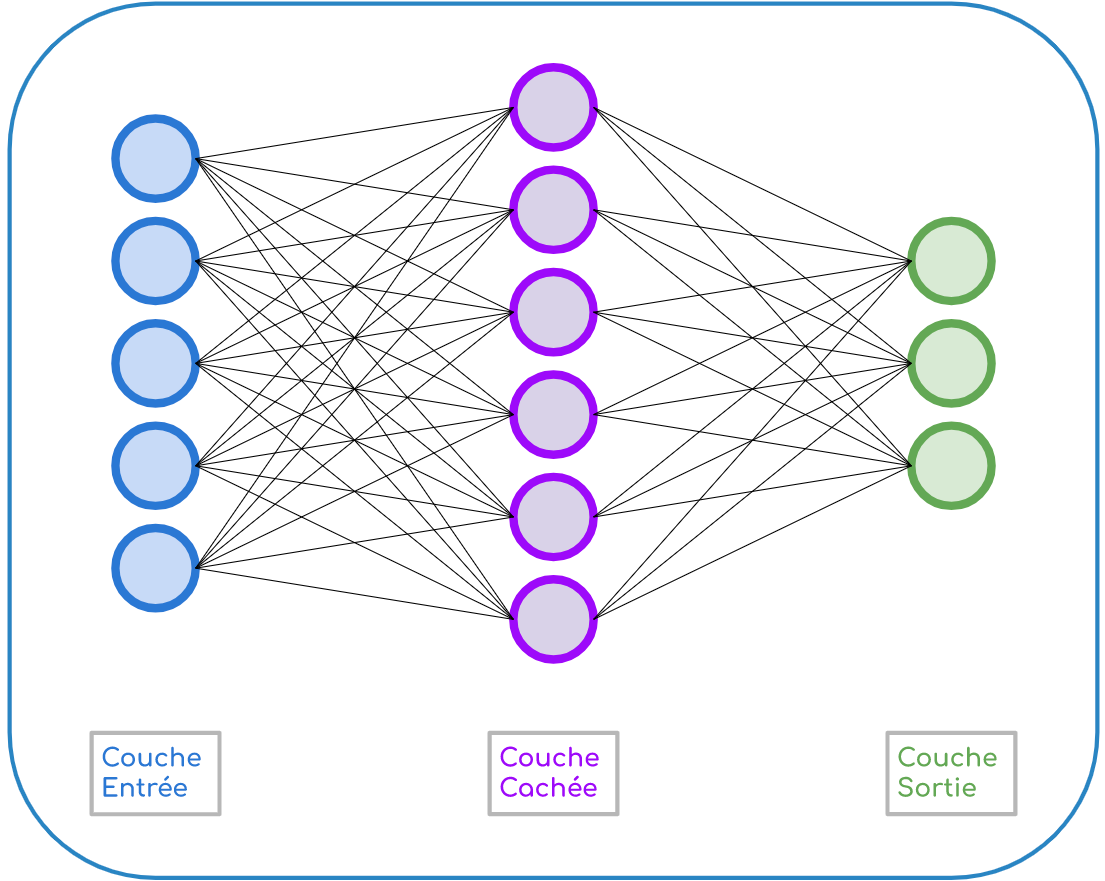
\includegraphics[width=0.8\textwidth]{multi_layer_perce.png}
            \caption{multi couche perceptron}
            \label{fig:m_l_p}
        \end{figure}

    \subsection{Réseau de neurones convolutionnel (RNC)}
    En apprentissage automatique, un réseau de neurones convolutifs (CNN ou ConvNet) est un type de réseau de neurones artificiels acycliques (feedforward) dont les schémas de connectivité entre les neurones sont inspirés du cortex visuel des animaux. Les neurones de cette zone du cerveau sont disposés pour correspondre à des zones qui se chevauchent lorsque le champ visuel est carrelé. Leur fonctionnalité s'inspire des processus biologiques et consiste en un empilement multicouche de perceptrons destiné à prétraiter de petites quantités d'informations. Les réseaux de neurones convolutifs ont un large éventail d'applications, notamment la reconnaissance d'images et de vidéos, les systèmes de recommandation et le traitement du langage naturel.

        \subsubsection{Architecture RNC standard}
        La forme la plus courante d'architecture de réseau neuronal convolutif empile plusieurs couches Conv-ReLU, suivies de couches de pool supplémentaires, répétant ce modèle jusqu'à ce que l'entrée soit réduite à un espace  suffisamment petit. À un moment donné, il est courant de mettre une couche entièrement connectée (FC). La dernière couche entièrement connectée sera connectée à la sortie. Vous trouverez ci-dessous une architecture de réseau neuronal convolutif commune qui suit ce modèle:

        \begin{figure}[H] 
            \centering
            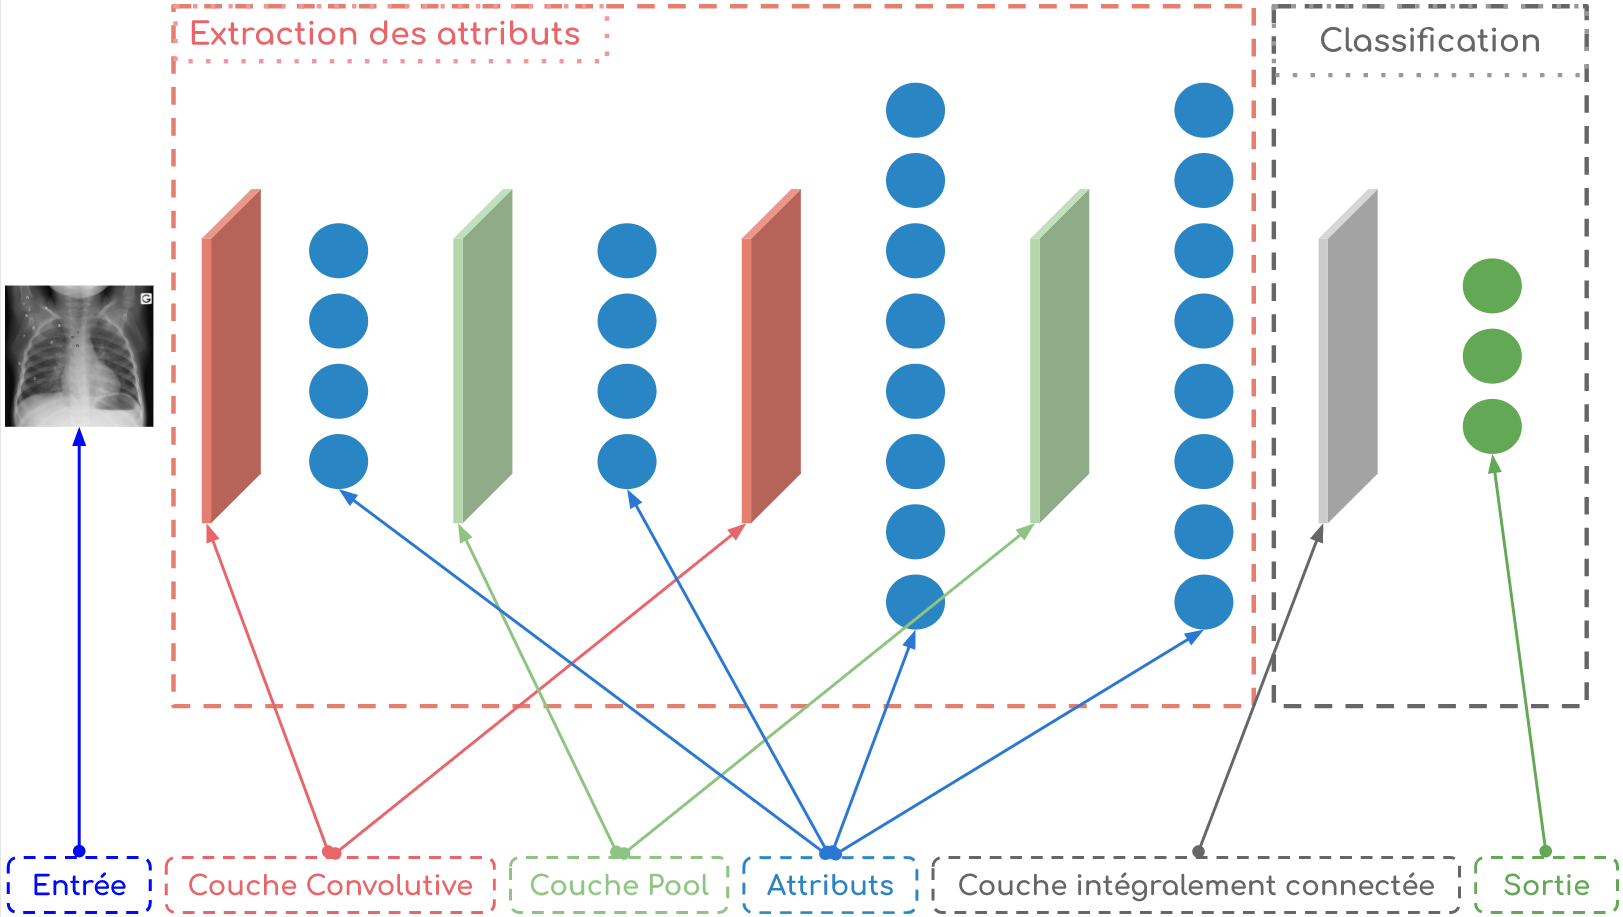
\includegraphics[width=\textwidth]{conv_stand_arch.png}
            \caption{Architecture standard d'un Réseau de neurones convolutionnel}
            \label{fig:conv_stand_arch}
        \end{figure}

        \subsubsection{Couche convolutive}
        Les couches convolutives sont à la base des CNN. Un paramètre de tranche consiste en un ensemble de filtres d'apprentissage (ou noyaux). Ces filtres ont un petit champ de vision, mais couvrent toute la profondeur du volume d'entrée. Dans le (Feed forward), chaque filtre est convolué sur la largeur et la hauteur du volume d'entrée et le produit scalaire entre les entrées du filtre est calculé pour produire la carte d'activation 2D pour ce filtre. Par conséquent, le réseau apprend quels filtres s'activent lorsqu'il détecte certains types d'entités à certains emplacements spatiaux dans l'entrée. 
        L'empilement des cartes d'activation de tous les filtres le long de la dimension de profondeur forme le volume de sortie complet de la couche de convolution. Chaque entrée dans le volume de sortie peut donc également être interprétée comme la sortie d'un neurone partageant des paramètres avec des neurones dans la même carte d'activation en regardant une petite région à l'intérieur de l'entrée.

        \subsubsection{Couche max pooling}
        Une couche max pooling est une nouvelle couche ajoutée après la couche de convolution. Surtout après avoir appliqué des non-linéarités (telles que ReLU)  aux cartes de caractéristiques générées par les couches convolutionnelles. 
        L'ajout d'une couche de max pooling après une couche convolutive est un modèle courant utilisé pour ordonner les couches dans les réseaux de neurones convolutifs qui se répètent une ou plusieurs fois dans un modèle particulier. 
        La couche max pooling fonctionne sur chaque carte d'entités indépendamment, créant un nouvel ensemble du même nombre de cartes d'entités regroupées.

        
        \subsubsection{Hyperparamètres}
        En apprentissage automatique, les hyperparamètres sont des paramètres dont les valeurs sont utilisées pour contrôler le processus d'apprentissage. En revanche, les valeurs des autres paramètres (généralement les poids des nœuds) sont obtenues par apprentissage. 
        Les hyperparamètres peuvent être classés comme des hyperparamètres de modèle qui ne peuvent pas être dérivés en ajustant une machine à un ensemble d'apprentissage, ou des hyperparamètres de modèle, car ils s'appliquent à la tâche de sélection de  modèle. Algorithmes qui, en principe, n'affectent pas les performances du modèle, mais affectent la vitesse et la qualité du processus d'apprentissage. Des exemples d'hyperparamètres de modèle sont la topologie et la taille du réseau neuronal. Des exemples d'hyperparamètres algorithmiques sont le taux d'apprentissage et la taille de la pile.
        \paragraph{Choix des hyperparamètres}
        Les réseaux de neurones convolutifs utilisent plus d'hyperparamètres que les perceptrons multicouches standards. Même si les règles habituelles de taux d'apprentissage et de constantes de régularisation s'appliquent toujours, les notions de nombre de filtres, leur forme et la forme du max pooling doivent être prises en considération.




\section{Classification des images}
    La classification des images est une tâche fondamentale qui tente de comprendre l'image dans son ensemble. Le but est de classer les images en leur attribuant des étiquettes spécifiques. La classification des images fait généralement référence aux images dans lesquelles un seul objet est affiché et  analysé. En revanche, la détection d'objets comprend à la fois des tâches de classification et de localisation et est utilisée pour analyser des cas plus réalistes où plusieurs objets peuvent être présents dans une image.

    Dans le domaine de la classification des images, nous avons exploré trois types bien connus:
    \begin{enumerate}
        \item Classification binaire
        \item Classification Multi-Classes
        \item Classification Multi-Etiquettes
    \end{enumerate}

    \subsection{Classification binaire}
        La classification binaire fait référence aux tâches de classification avec deux étiquettes de classe. 
        Les tâches de classification binaire ont généralement une classe représentant les conditions normales et une autre classe représentant les conditions anormales. 
        Et dans notre cas, dans l'image, on fait référence à la présence d'objets (en prenant l'étiquette 0) ou non (en prenant l'étiquette 1).
    \subsection{Classification Multi-Classes}
        Contrairement à la classification binaire, la classification multi-classes n'a pas la notion de résultats normaux et anormaux. Au lieu de cela, les exemples sont classés comme appartenant à l'une parmi une gamme de classes connues.

        Le nombre d'étiquettes de classe peut être très important sur certains problèmes. Par exemple, un modèle peut prédire qu'une photo appartient à un parmi des milliers ou des dizaines de milliers de visages dans un système de reconnaissance faciale.

        Mais la chose la plus importante à noter est que le résultat prédit de ce modèle est une classe unique qui le rend moins intéressant dans notre cas où une radiographie peut avoir de multiples anomalies.
    \subsection{Classification Multi-Etiquettes}
        Ceci est différent de la classification binaire ou multiclasse, où une seule étiquette de classe est prédite par instance. 
        Il est courant de modéliser des tâches de classification multi-étiquettes à l'aide de modèles qui prédisent plusieurs sorties, où chaque sortie est prédite sous la forme d'une distribution de probabilité de Bernoulli. Il s'agit essentiellement d'un modèle qui effectue plusieurs prédictions de classification binaire par exemple. 
        Les algorithmes de classification utilisés pour la classification binaire ou multiclasse ne peuvent pas être utilisés directement pour la classification multiétiquette. Une version spéciale de l'algorithme de classification standard est disponible, appelée version multi-étiquettes de l'algorithme:
        \begin{itemize}[label=$\bullet$]
            \item Arbres de décision multi-étiquettes
            \item Forêts aléatoires multi-étiquettes
            \item Amplification des dégradés multi-étiquettes
        \end{itemize}


\section{Apprentissage par transfert}
    L'apprentissage par transfert est la réutilisation de modèles pré-entraînés pour de nouveaux problèmes. Il est actuellement très populaire  en apprentissage profond car il permet d'entraîner des réseaux de neurones profonds avec relativement peu de données. Ceci est très utile dans le domaine de la science des données. En effet, la plupart des problèmes du monde réel n'ont généralement pas des millions de points de données étiquetés pour entraîner un modèle aussi complexe.


\section*{Conclusion}
        Ce qu'on peut en deduire de ce chapitre c'est que pour la réussite de notre projet on doit se baser sur 3 concept principales:
        \begin{enumerate}
            \item Réseaux de neurones convolutifs
            Pour le traitement des données qui ont sous forme de clichés de radiologiques (images)
            \item Classification Multi-Etiquettes
            Car on veut que le modèle détecte tout les anomalies possible non seulement une.
            \item Apprentissage par transfert
            On a pas assés de données pour crée un modèle puissant donc on va se baser sur un modèle pré-entraîné, pour assurer une bon précision avec le minimum de données.
        \end{enumerate}